\documentclass{article}


\usepackage{arxiv}

\usepackage[utf8]{inputenc} % allow utf-8 input
\usepackage[T1]{fontenc}    % use 8-bit T1 fonts
\usepackage{hyperref}       % hyperlinks
\usepackage{url}            % simple URL typesetting
\usepackage{booktabs}       % professional-quality tables
\usepackage{amsfonts}       % blackboard math symbols
\usepackage{nicefrac}       % compact symbols for 1/2, etc.
\usepackage{microtype}      % microtypography
\usepackage{lipsum}
\usepackage{graphicx}
\usepackage[russian]{babel}
\usepackage{pgfplots}
\usepackage{layout}
\usepackage{amsmath}

\graphicspath{{rcs/}}

\title{Построение индекса сентиментов для анализа рынка акций}

\author{
  Бучко Даниил Владимирович \\
  Факультет Экономических Наук\\
  Студент, 3-ий курс бакалавриата \\
  НИУ ВШЭ, г. Москва\\
  \texttt{dvbuchko@edu.hse.ru} \\
  %% examples of more authors
   \And
 Соколова Татьяна Владимировна \\
  Факультет Экономических Наук \\
  Старший преподаватель \\
  Базовая кафедра инфраструктуры финансовых рынков \\
  Аналитик в ЛАФР, НИУ ВШЭ, г. Москва \\
  \texttt{tv.sokolova@hse.ru} \\
  %% \AND
  %% Coauthor \\
  %% Affiliation \\
  %% Address \\
  %% \texttt{email} \\
  %% \And
  %% Coauthor \\
  %% Affiliation \\
  %% Address \\
  %% \texttt{email} \\
  %% \And
  %% Coauthor \\
  %% Affiliation \\
  %% Address \\
  %% \texttt{email} \\
}

\begin{document}
\maketitle

\begin{abstract}

Когда заинтересованный исследователь попадает на финансовый рынок, для него открывается множество инструментов для принятся инвестиционных решений. Все эти инструменты в основе своей базируются на двух основновополагающих источниках: на фундаментальной и технической информации. Использование данных из этих источников подразумевает не только первичную обработку, но и последующую интерпертацию полученных результатов, что является достаточно трудозатратным процессом. А что если есть иные источники информации, которые могут передавать содержательный смысл анализа общедоступных данных? Что если направлять усилия не на исследования состояния определенной компании, а попробовать прислушаться к тому, что говорят люди об этой компании? Может быть у нас получится получить общее представление о состоянии компании, основываясь на разрозненные мнения? В данном исследовании я проведу анализ альтернативных источников принятия решений и проверю их эффективность на примере российского рынка акций. В качестве таких источников будут выступать форумы и телеграм каналы.


\end{abstract}


% keywords can be removed
% \keywords{First keyword \and Second keyword \and More}


\section*{Вступление}
Я бы хотел провести читателя этой статьи по пути вопросов и ответов, которые возникают сами собой в ходе решения любой поставленной задачи. Поэтому, сформулируем первый логичный вопрос: 
<<\emph{Что мы хотим сделать?}>>. Как было сказано раннее в асбстракте, мы бы хотели получить полезную информацию о компаниях, торгующих ценными бумагами, не прибегая к трудозатратным операциям, предполагающим знания финансовой отчетности или технического анализа. Следующий логичный вопрос: <<Что это за информация и почему её можно считать ценной?>> Частично на этот вопрос мы ответим в главе 1, где планируется выбрать данные и определиться с их источниками, а частично $-$ в главе 4, где определимся с тем, насколько ценной оказалась полученная информация. В главе 1 я также рассмотрю особенности и способы получения данных. Будет показано на примерах, как выглядит структура источников, каким образом осуществляется автоматический сбор и обработка данных. Затем полученные данные мы начнем активно исследовать в главе 2, чтобы ответить на следующий вопрос: <<Как использовать полученные данные?>> При подробном расммотрении я опишу основные тонкости и механизмы предобработки полученных текстов, покажу особенности конкретно наших данных, посчитаю статистики и визуализирую основные результаты. В главе 3 мы займемся вопросами непосредственного моделирования языка при помощи машинного обучения и нейронных сетей: сформулируем задачу, выберем метрики, а затем подберем подходящую модель. 



\section{Получение данных.}
\label{sec:headings}



\subsection*{Какие данные использовать?}

Информацию об окружающем мире можно черпать из различных источников. Очевидно, что любой источник информационного потока имеет свои особенности и отличительные черты. К примеру, информация, публикуемая в журналах, обычно проходит через долгие корректировки, и к моменту выпуска издания, она может частично или полностью искажаться, утрачивать свою значимость и актуальность, в зависимости от задачи, в которой эта информация планировалась использоваться. Аналогичными свойствами можно охарактеризовать информацию, получаемую из новостей, регулярных аналитических сводок и стриминговых сервисов. Более того, важной отличительной чертой всех этих источников является то, что информация, получаемая на выходе, проходит через множество рук и любые конкурентные приемущества связанные с ценностью новой информации могут быть утеряны, потому что всегда будет некий посредник между исследователем и событиями.  
\par Поэтому, для нашей задачи,$-$ оперативно получать потенциально полезную информацию о финансовом рынке $-$ необходимо выбрать источники, обладающие подходящими свойствами:

\begin{enumerate}
	\item Релевантность. Важнее всего, чтобы информация с нашего источника имела отношение к ценным бумагам и гипотетически имела предсказательную силу. Ведь именно для этого мы и собираемся её собирать и обрабатывать. Отсекаем любые неэкономические источники данных.
	\item Доступность. Это свойство позволит оперативно получать факты об изменениях на рынке без дополнительных ограничений, накладываемых посредниками или высокими издержками.  Исключаем источники данных, за которые необходимо платить. 
	\item Высокая частотность данных. Очень удобно выбирать такой источник, информация с которого была бы в достаточном количестве, для проведения простейшего статистистического анализа. Кроме этого, это свойство дает возможность моментально адаптироваться к любым шокам, меняющим конъюктуру рынка ценных бумаг. Концентрируемся на постоянно обновляющихся, высокочастотных источниках данных.
\end{enumerate}
Учитывая все аспекты, приведенные выше, я решил остановиться на текстовых источниках данных. Релевантность кокретизируется в текстовых данных, описывающих ситуацию на рынке акций. Как быть с доступностью? Здесь можно выбрать источники, не требующие денежных и временных издержек на ожидание получения информации $-$ финансовые форумы и группы в социальных сетях. Заметим, что такие источники удовлетворяют и последнему свойству $-$ свойству высокой частотности. Многие онлайн-платформы, ставшие привычным местом для обсуждения инвестиционных идей и стратегий существуют на российском рынке аж с конца 2000-х годов и активно развиваются по сей день.

\subsection{Интернет сообщества: сайты}

Безусловным лидером на на российском рынке финансовой информации является интернет платформа \href{www.mfd.ru}{MFD}. Судя по информации об интернет-ресурсе\footnote{https://mfd.ru/about/}, эта платформа работает с $1996$ года и объединяет ежедневно более $10000$ человек.
Вторым кандидатом на подходящий источник информации является интернет сообщество \href{https://smart-lab.ru}{Smart-Lab}. Помимо указанных ресурсов, существует несколько интересных организаций, предоставляющих финансовую информацию, среди них: \href{http://cbonds.ru}{Cbonds}, \href{https://quote.rbc.ru}{Quote РБК}, \href{https://investfunds.ru}{InvestFunds}. 
Единственное отличие последних состоит в том, что они работают по принципу предоставления контента, а значит не до конца удовлетворяют нашей предпосылке о доступности. Остановимся на MFD.

\subsection{Интернет сообщества: телеграм каналы}
Телеграм-каналы стали популярны на пике введения блокировок в результате отказа основателя компании от предоставления ключей шифрования государству\footnote{https://www.sostav.ru/publication/telegram-38688.html}. Сложно судить, что стало ключевым фактором в успехе телеграма, будь то зажигающая идея противостояния государству, которую так любит молодежь, либо удобный интерфейс, но телеграм полюбили и не обошли стороной люди, имеющие непосредственное отношение к финансовым рынкам. Так или иначе, телеграм предоставляет удобный и простой способ обсуждения различных тематик, поэтому заприметим этот источник информации как задел на будущие исследования и вернемся к его обсуждению в заключительной секции этого исследования. 
\par Итак, мы разобрались с тем, что интернет площадка MFD обладает всеми необходимыми для нашего исследования характеристиками. Следующий вопрос: <<Какую конкретно информацию, мы собираемся использовать?>>. Существуют многочисленные исследования в области анализа влияния текстовой информации на изменение в доходности ценных бумаг\footnote{Работы [1], [2], [3] в списке литературы}. В данных исследованиях проверялась гипотеза о влиянии социальных сетей на доходность акций и индексов. Более того, были предприняты успешные попытки построить регрессионные модели, объясняющие доходность индексов, ориентируясь только на сентименты сообщений в социальных сетях. Попробуем сделать подобное исследование, но с использованием более современного подхода в области моделирования языка и на российском рынке акций.

\subsection{Сбор информации с интернет-ресурсов}
Поскольку мы определились с тем, что и откуда будем собирать, настало время понять, каким образом выполнить эту задачу. Для этого нужно получить представление о строении сайтов и понять, из каких деталей состоят веб-страницы. Ниже можно видеть переписку участников финансового форума в той форме, в которой её видит человек и в том обличии, в каком она предстает перед браузером. 
\begin{figure}[h]
	\center{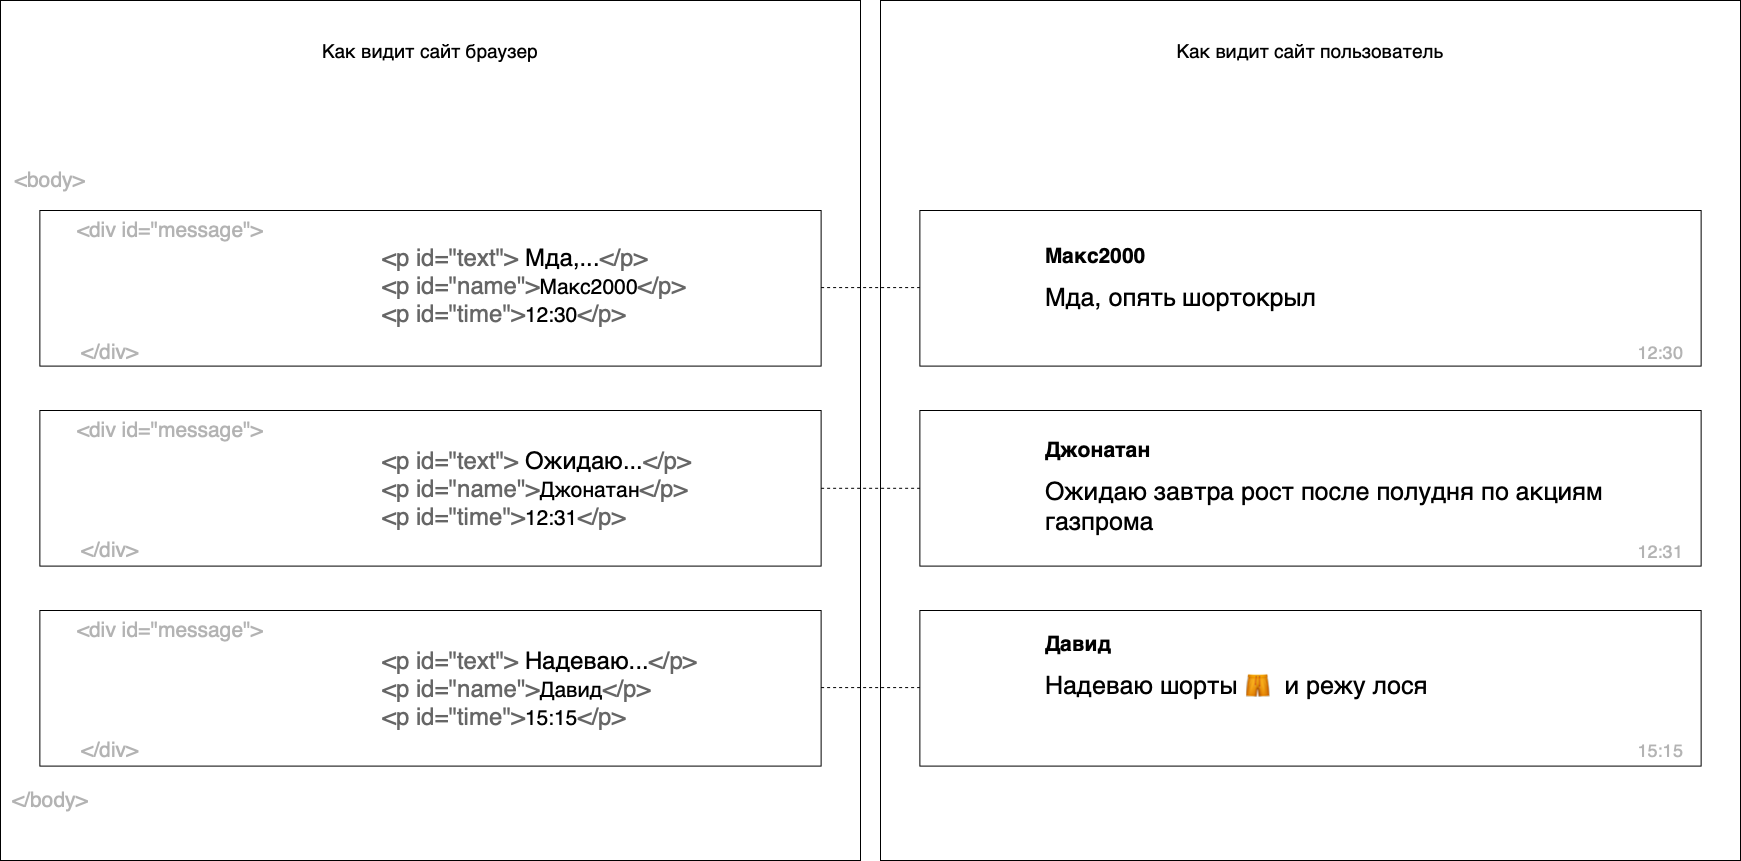
\includegraphics[scale=0.27]{html.png}}
	\caption{Каким образом информация предоставлена на сайте}
	\label{fig:image}
\end{figure} \\
Заметим, что каждое сообщение находится в соответствующем блоке (контейнере). Таким блокам присваивается метка <<message>>, явно указывающая на содержимое контейнера. Весь процесс сбора данных состоит в том, чтобы отыскать все контейнеры на странице, получить их содержимое и перейти к следующей странице. Обратим внимание на то, как хорошо структурирована информация на этом примере. В реальности сайты редко бывают статическими, обычно они меняют свою структуру под воздействием пользовательский действий. Но это явно не случай российских форумов, написанных с конца 90-х годов. Кроме того, нужно с осторожностью пользоваться автоматическим сбором данных. Некоторые сайты запрещают использование парсеров, потому что слишком частые запросы страниц нагружают сервера и неправильно написанный код может значительно затруднить пропускную способность интернет-ресурса. Переходим к следующему шагу. \\

\begin{table}[h]
	\caption{Примеры полученных сообщений}
	\centering
	\begin{tabular}{llp{9.45cm}l}
		\toprule
		Дата сообщения     &  Имя пользователя    & Текст сообщения  \\
		\midrule
		09.11.2014 15:46     & Веном  & ШОРТИТЕ!!!		\\
		09.11.2014 17:17     & михаил2 & ты первый	      \\
		09.11.2014 17:43     & петрович       & Так вы будете бить рекорд погружения или как?  \\
		09.11.2014 18:09     & Веном  & Рубль непоколебим в России.  Доллар растёт		\\
		09.11.2014 18:27     & capitan & Начинайте	мне еще пару тысяч прикупить надо...	      \\
		10.11.2014 14:33     & capitan       & Прикупил себе PLZL.  \\
		10.11.2014 15:47     & capitan       & Главное не слейся раньше времени	как на Алросе) хотя я и сам так сделал)  \\
		10.11.2014 16:37   & драконорожденный       & Не	не сольюсь.    А с Алросой я ошибку сделал. Надо было смотреть на то \\    
		11.11.2014 11:36     & драконорожденный       & Думаю	что эту цену мы увидим не раньше следующей весны...Я предупреждал \\    
		
		14.11.2014 22:52   & МарКс       & Все после таких новостей понятно стало \\    
		15.11.2014 22:59     & трейдерсрублевки       & http://oilru.com/news/436599/	 \\    
		\bottomrule
	\end{tabular}
	\label{tab:table}
\end{table}

\section{Подготовка данных}
В результате сбора данных были получены сообщения с 2008 по 2020 год по компаниям из разных групп капитализаций: маленькие, средние и большие. (см. примеры Таблица \ref{tab:table}). Перед тем, как перейти к процессу построения моделей, необходимо предобработать текст таким образом, чтобы максимально исключить всю лишнюю информацию. Для этого текст, при помощи регулярных выражений, очищается от любой пунктуации, любых небуквенных символов, лишних пробелов и неинформативных ссылок и слов. После этого, каждое предложение приводится к нижнему регистру, лемматизируется (то есть приводится к своей начальной форме) и стеммингуется (обрезается таким образом, чтобы от слова осталась только его основа). Произведенные операции позволяют сократить количество неиформативных признаков, тем самым улучшая скорость и точность работы оптимизационных алгоритмов. В результате подобной обработки, сообщения стали иметь следующий вид:

\begin{table}[h]
	\caption{Сообщения после обработки}
	\centering
	\begin{tabular}{llp{9.45cm}l}
		\toprule
		Дата сообщения     &  Имя пользователя    & Текст сообщения  \\
		\midrule
		09.11.2014 15:46     & Веном  & шорт		\\
		09.11.2014 17:17     & михаил2 & ты	перв    \\
		09.11.2014 17:43     & петрович       &  так вы быт бит рекорд погружен ил как   \\
		09.11.2014 18:09     & Веном  & рубл непоколебим в росс доллар раст	\\
		09.11.2014 18:27     & capitan & начина я ещ пар тысяч прикупа	      \\
		10.11.2014 14:33     & capitan       & прикупа себ plzl  \\
		10.11.2014 15:47     & capitan       & главн не слива ран врем как на алрос хот я и сам так сдела  \\
		10.11.2014 16:37   & драконорожденный       & не не слива а с алрос я ошибк сдела быт смотрет на то \\    
		11.11.2014 11:36     & драконорожденный       & дума что этот цен мы увидет не ран след весн я предупрежда \\    
		
		14.11.2014 22:52   & МарКс       &  посл так новост понятн станов \\    
		15.11.2014 22:59     & трейдерсрублевки       &  	 \\    
		\bottomrule
	\end{tabular}
	\label{tab:table2}
\end{table}

Обратим внимание на то, что сообщения в большинстве случаев не потеряли свой основной смысл, однако количество уникальных слов сократилось в 4 раза: с $131,530$ до $34,733$. Такой подход в обаботке текстов имеет свои ограничения, и иногда останавливаются на этапе лемматизации, но как мы увидим далее, именно такой способ подготовки сообщений позволит делать наиболее точные прогнозы в рамках конкретно нашей задачи. В приложении можно посмотреть на другие интересные статистики по датасету (см. Главу \ref{chap:additional}).

\begin{figure}[h]
	\centering
	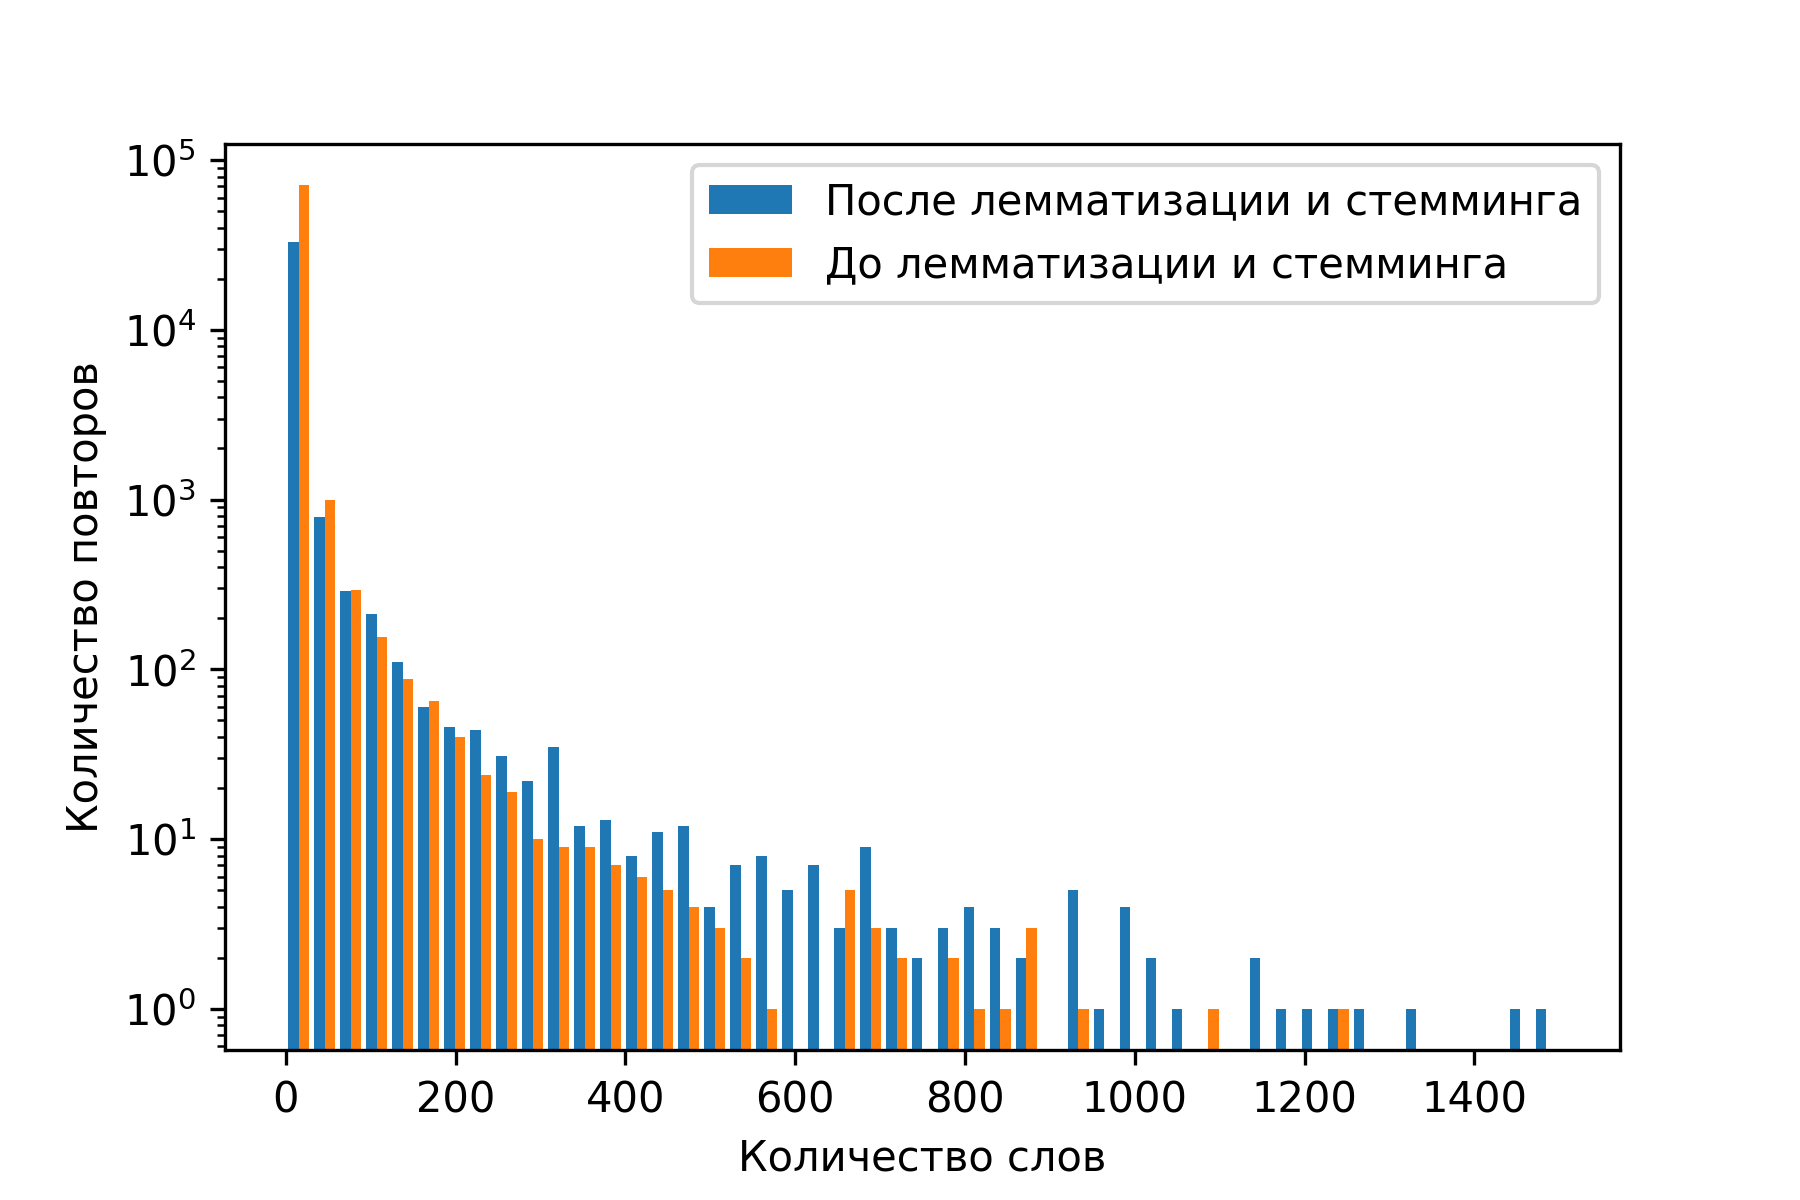
\includegraphics[scale=0.65]{before_after.png}
	\caption{Распределение слов в тренировочном наборе данных}
	\label{pic:dist}
\end{figure}

Как можно видеть из рисунка \ref{pic:dist}, в результате обработки данных частотность слов распредилилась более равномерно, уменьшая долю выбросов в выборке. На изображение не попали слова с очень низкой частотностью, для сохранения наглядности. В приложении есть таблица \ref{tab:table4}, показывающая примеры частоупотребляемых и редкоупотребляемых слов. Переходим к выбору модели.

\section{Выбор модели}
Следующий момент, который мы должны для себя решить $-$ как использовать собранные данные? В работах \cite{2014oli}, \cite{2017ren} авторы предпринимали попытки объяснить доходность бумаг, исходя из гипотезы, которую можно сформулировать следующим образом: <<Эмоциональный фон, складывающийся вокруг определенной бумаги, влияет на решение инвестора (по крайней мере частного) о покупке или продаже той или иной бумаги>>. Для того чтобы проверить эту гипотезу, нам необходимо построить модель $F(.)$, которая бы переводила сообщения во множество эмоциональных признаков по следующей схеме:

\begin{equation}
\label{eq:F}
F(\text{сообщение}) = 
\begin{cases}
3, &\text{если сообщение носит позитивный окрас}\\
2, &\text{если сообщение не относится к финансовому рынку} \\
1, &\text{если сообщение носит негативный эмоциональный окрас} \\
\end{cases}
\end{equation}

Получается, что для нас, как для исследователей, задача сводится к построению модели, разделяющей все сообщения на 3 группы. С точки зрения машинного обучения, такая задача именуется задачей классификации. Выделим ключевые особенности нашего набора данных, чтобы выбрать подходящую модель:

\begin{enumerate}
	\item Изменчивость лексики во времени. Некоторые фразы, под влиянием различных культурных особенностей, меняют со временем то, как мы выражаем свои мысли, поэтому из всего количества собранных данных, для обучения были взяты сообщения из различных временных промежутков.
	\item Постобработанные данные не имеют меток класса. Простым языком, чтобы использовать алгоритмы обучения с учителем, нам необходимо дополнительно вручную разметить данные. Особенности рутинной ручной разметки ограничивают количество данных для обучения, поэтому из этого пункта возникает следующая характерная черта.
	\item Относительно небольшой датасет. В результате разметки совместными усилиями с группой единомышленников был сформирован итоговый датасет, состоящий из $30,000$ наблюдений.
	\item Несбалансированность классов. Очень важная черта, которую обязательно необходимо иметь в виду, при построении любой модели. В наших данных после разметки, распределение классов имело вид, изображенный на рисунке 	\ref{pic:imb}
\end{enumerate}

\begin{figure}[h]
	\centering
	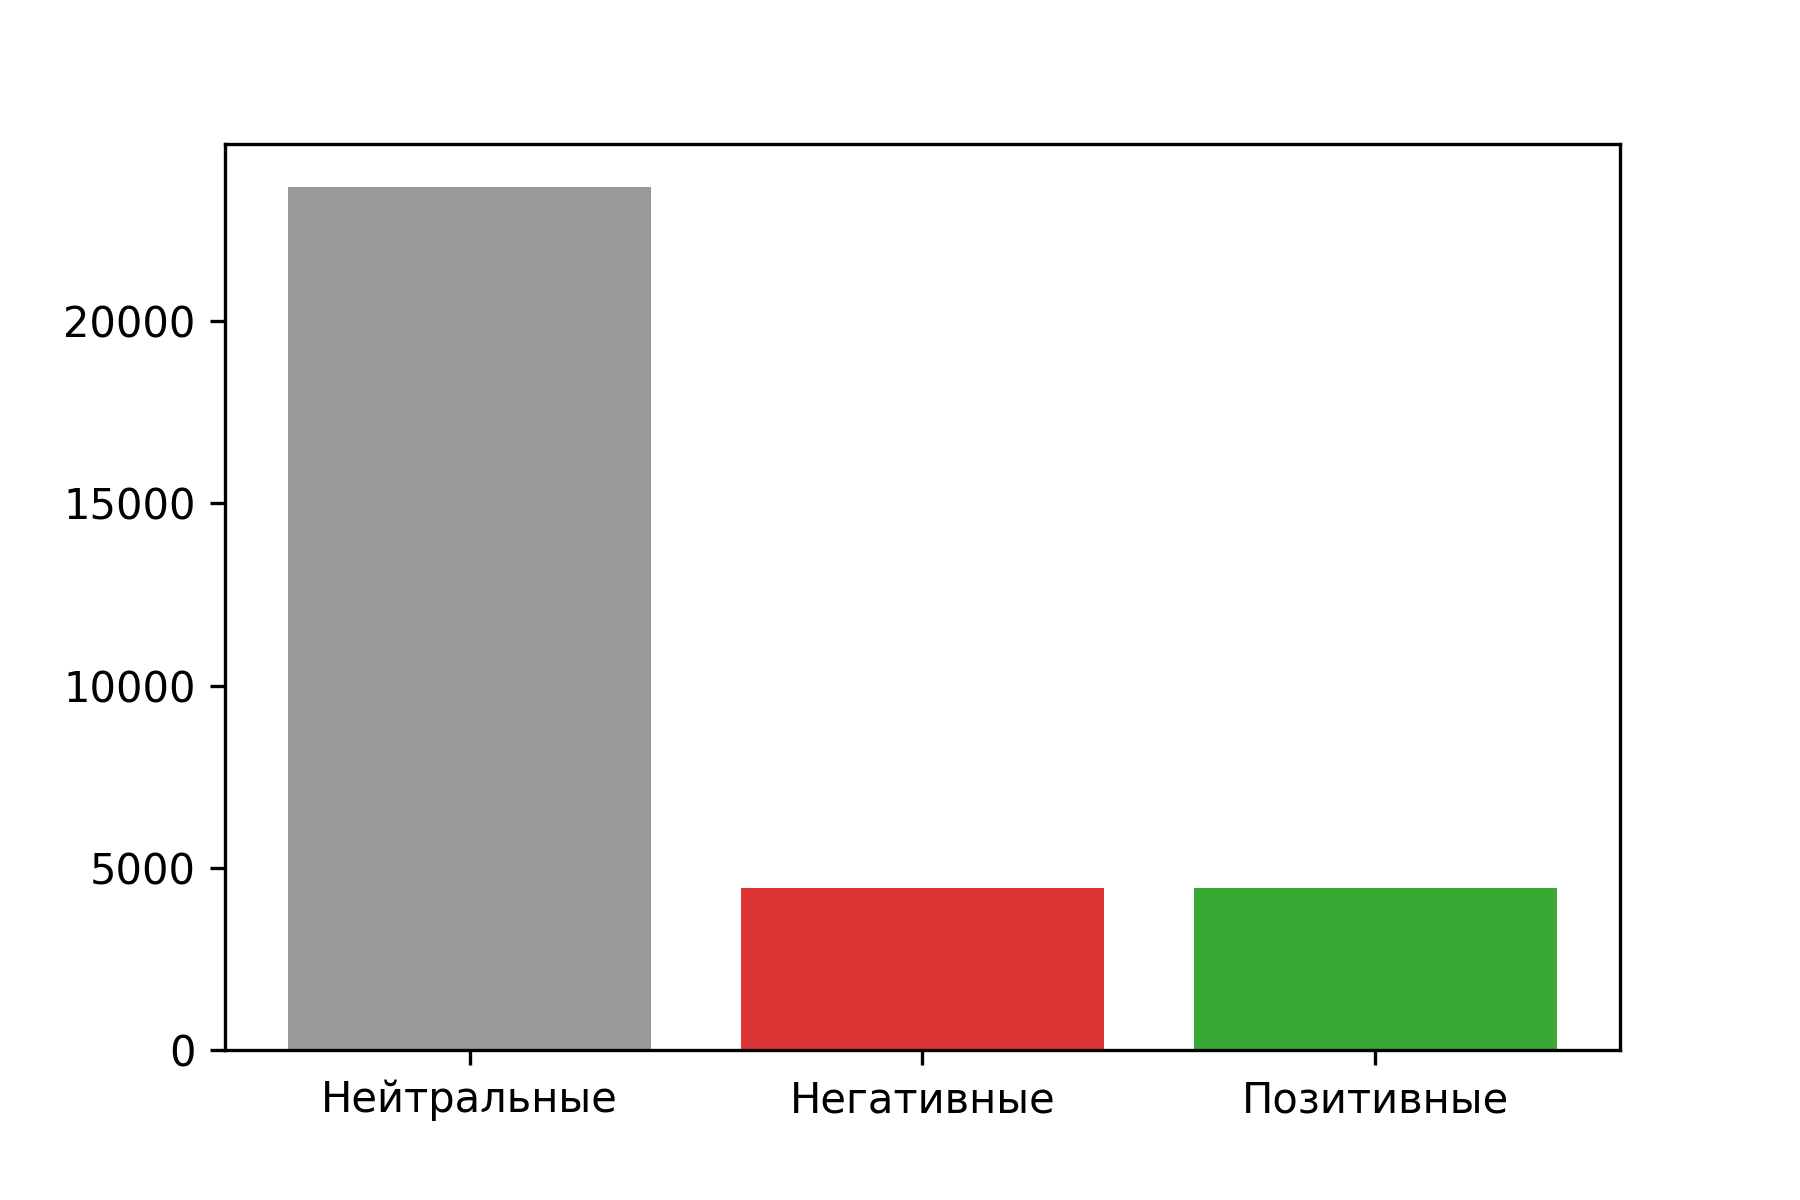
\includegraphics[scale=0.65]{imbalance.png}
	\caption{Распределение категорий в тренировочном наборе данных}
	\label{pic:imb}
\end{figure}

Особенности 3-4, обсуждаемые выше, будут активно приниматься во внимание при построении моделей.

\subsection{Представление данных}
Чтобы построить классификатор сообщений, нужно представить данные, понятным компьютеру образом. Более формально, нам необходимо определить пространство, из которого искомая модель $F(.)$ будет переводить сообщения в соответсвующие сентиментам классы. Имея численное представление каждого из предложений, можно применять математический аппарат к построению моделей. Принимая во внимание методы машинного обучения и статистики, такие представления могут задаваться самыми различными способами. В ходе исследования мы будем постепенно двигаться от простейших к более продвинутым, попутно делая выводы о преимуществах и недостатках каждого из подходов.

\subsubsection{OneHotEncoding}

OneHotEncoding $-$ один из множества способов определения множества значений, на котором будет работать искомая модель $F()$. Суть метода заключается в создании дамми-переменных в количестве, равном количеству слов в датасете. Таким образом, каждое сообщение можно закодировать вектором, состоящим из нулей и единиц. Единицы будут характеризовать наличие определенного слова, а нули $-$ отсутствие. Такой подход накладывает свои ограничения, среди которых:

\begin{enumerate}
	\item Необходимость хранения в оперативной памяти большого объема данных в процессе обучения алгоритма. В нашем случае, размер датасета, закодированного таким образом, имел бы размерность \[R^{\text{ Количество сообщений }\times\text{ Количество слов}} = R^{~31000\times 34733}\]
	\item Учитывая, что каждое слово кодируется единицей, получаем, что все слова имеют одинаковый вес. Однако, в русском языке некоторые слова встречаются гораздо чаще других, и их большее количество в тренировочных данных будет накладывать отпечаток на процесс оптимизации, о котором речь пойдет ниже. В качестве шага предобработки были предприняты меры по уменьшению количества лишних слов, но как можно видеть в таблице \ref{tab:table4}, среди наиболее употребительных слов все еще мелькают слова, не влияющие на сентимент сообщения.
\end{enumerate}

\subsubsection{Tf-Idf Encoding}
Tf-Idf $-$ решение проблемы равновзвешивания слов в процессе моделирования связи между сообщениями и их эмоциональным окрасом. Согласно этому подходу, каждому уникальному слову в тренировочном наборе данных соответствует определенный вес, исчисляемый по специальной формуле. Взвешивание слов должно решать главную проблему $-$ уменьшать значимость слов, которые не несут практического смысла. Как определить какое слово несет смысл, а какое нет? Создательница\footnote{Karen Spärck Jones. Synonymy and Semantic Classification — Edinburgh University Press., 1986. — Vol. 1. — (Edinburgh Information Technology series)} TF-IDF предложила следующую идею: если слово характерно не только для определенного сообщения, а для всего датасета в целом, то скорее всего, оно несет меньшую смысловую нагрузку, чем слово, которое встречается только в одном сообщении датасета. Чтобы отделить такие слова друг от друга, она придумала статистику, под названием TF-IDF, которая состоит из двух частей: TF (Term Frequency) и IDF (Inverse Document Frequency) и считается для каждого слова в отдельности. \[\text{TF-IDF}_{\text{i}} = TF_{\text{i}} \times IDF_{\text{i}} \quad \forall i  \text{ из словаря всех слов}\]
$TF_{i}$ часть отвечает за важность слова в пределах одного сообщения и рассчитывается по следующей формуле: \[ TF_{i} = \frac{n_{i}}{\sum_{k=1}^{n}n_k} \]
где $n_i -$ количество повторений i-го слова в сообщение, а $n_k - $количество слов в одном сообщении.\\
$IDF_i$ отвечает за значимость слова в контексте всех сообщений в том смысле, о котором говорилось ранее: \[ IDF_i = \log \frac{|D|}{|{\{d_t \in D | i \in d_t\}}|}\] 
где $|D| - $количество всех сообщений, а $|\{d_t \in D | i \in d_t\}| - $количество сообщений, в которых встретилось i-ое слово. 
Получается, что для каждого слова мы считаем величину IDF, которая является единой для одинаковых слов и TF, которая разнится от предложения к предложению. Величина $TF-IDF$ тем больше, чем характернее слово для каждого из предложений. Среди проблемных мест такого численного представления слов можно выделить следующий:

\begin{enumerate}
	\item При кодировании теряется значение слов, определяемое порядком. К примеру, для TF-IDF, равно, как и для OneHotEncoding не существует разницы между предложениями <<Здесь сложно придумать что-то совершенно не бессмысленное>> и  <<Здесь не сложно придумать что-то совершенно бессмысленное>>.
\end{enumerate}

Разобравшись с возможностями представления слов в численном виде, мы смогли наглядно увидеть, как можно подготовить текстовые данные к тому, чтобы начать оценивать заветную модель \hyperref[eq:F]{(1)}. Настала пора перейти к самой интересной\footnote{Когда я проходил стажировку в одной из компаний занимающихся Data-Science, мой руководитель любил говорить, что выбор модели - награда за долгую и рутинную работу по предобработке данных.} части нашего исследования $-$ подбору модели. \\
Одно из негласных правил хорошего тона при любых исследованиях в сфере машинного обучения $-$ начинать с простейших моделей. Эта идея понятна: чем сложнее задача, чем сильнее желание попробовать что-то из ряда вон выходящее, но при рассмотрении сложных моделей, требующих более тонкой надстройки, исследователи, занимающиеся процессом оптимизации, зачастую не понимают, как хорошо работает их алгоритм. Можно видеть значения точности в районе $70\%$ успешно классифицируемых сообщений, однако совершенно непонятно, является ли это значение наилучшим, или, может быть, необходимо тратить кучу дополнительного времени на сбор дополнительных сообщений и их последующей разметки\footnote{Andrew Ng - известный исследователь в области машинного обучения и нейронных сетей. Его видеокурсы доступны на платформе coursera.org. На одной из своих лекций он рассказывал о компаниях, занимающихся применением ИИ в своих разработках, которые обращались к профессору за консультациями по исследованиям. Разработчики рассказывали о задаче, об алгоритмах которые они применяли, о результатах оптимизации и находились серьезные компании, которые не могли понять, почему их модели выходят на плато по точности и огромные временные и денежные затраты по добыче новых данных не исправляют проблем. Решением подобных ситуаций оказывалось сравнительная конкурентоспособность продвинутых алгоритмов с простейшими моделями. Руководители ИИ компаний, используя простейшие алгоритмы, получали бэнчмарки, нижние пороги по качеству моделей и понимали, что правильное направление - дооптимизация существующих алгоритмов.}. Начнем выбор модели с основных понятий. \\
\subsubsection{Основные понятия}
Подбор модели осуществляется в три этапа:
\begin{enumerate}
	\item Выбор оптимизируемой функции потерь. Эта специальное название функции, которая нужна, чтобы понимать, как хорошо наша модель отражает моделируемую зависимость. Функция потерь позволяет обучать алгоритмы.
	\item Выбор метрики качества. Эта метрика необходима, чтобы сравнивать между собой различные алгоритмы и интерпретировать потенциал обученной модели.
	\item Выбор непосредственно модели. Модель $-$ попытка формального построения связи между объектами исследования.
\end{enumerate}

\subsubsection{Функция потерь}
В парадигме подхода машинного обучения, подбор модели, отражающей исследуемую зависимость, осуществляется на основе постоянных наблюдений за влиянием изменений параметров модели на качество предсказания. Простыми словами, мы каким-то образом перебираем набор моделей и пытаемся понять, как хорошо та или иная модель отражают действительность. Учитывая особенности конкретно нашей модели (\ref{eq:F}), нам нужно учитывать, что сама модель переводит сообщения из некоторого пространства произвольной рамерности в 3-х мерное пространство эмоциональных состояний. В идеале, нам нужно предсказывать вероятности каждого из классов, причем предсказания каждого из классов образуют полную группу событий. Поэтому, избираемая функция потерь должна учитывать эту особенность. Кроме этого, вспомним об особенностях наших данных, заключающихся в несбалансированности классов. На такие запросы теория машинного обучения предлагает следующую функцию: \[ Loss(y, \hat{p}) = - \sum_{c=1}^{3} w_c y_c log(\hat{p}_c), \quad \text{где}\]
$w \in R^3 - $ вектор весов. \\
$y \in R^{3} - $ бинарный вектор метки класса определенного сообщения \\ $\hat{p} \in R^3 - $ вектор предсказания вероятностей сентимента для определенного сообщения \\\\
Напомню, что размерность вектора ответов для предсказываемого сообщения равна 3, потому что мы предсказываем вероятности каждого из 3-х классов сентимента. Вектор весов будет учитывать ошибку, совершаемую на несбалансированном классе сильнее, чем на доминирующем, чтобы мы не делали поспешных выводов о моделях с низкой функцией потерь, постоянно предсказывающих доминирующий класс. Итак, подытожим: процесс обучения будет сводиться к оптимизации функции потерь, путем перебора различных моделей. Чем меньше вероятность верного класса, тем выше значение функции потерь.

\subsubsection{Метрика качества}
Хорошая метрика качества должна оценивать предсказательную силу модели и давать ей интерпретацию. В случае многоклассовой классификации, предлагается следующий набор метрик:
\begin{enumerate}
	\item \emph{Accuracy} - показатель средней точности распознавания класса. Его основной недостаток заключается в отсутсвии чувствительности к несбалансированности. Высчитывается по следующей формуле: $\begin{aligned}[t]
	Accuracy(y, \hat{y}) = \frac{1}{n} \sum_{i=1}^{n}[y_i = \hat{y}_i]
	\end{aligned}$
	\item F-мера
\end{enumerate}



\section{Тестирование полученной информации}
dwadlwmdmawd

\section{Приложение}
adownawdnaodin

\label{chap:additional}

\begin{table}[h]
	\caption{Частотность первых и последних 20 слов после обработки}
	\label{tab:table4}
	\centering
	\begin{tabular}{llll}
		\toprule
		%Заголовки
		Слово & Частотность слова &Слово & Частотность слова\\
		\midrule
		не & 13517 & marketbeat & 1\\ 
		а & 6964 & bmo & 1\\ 
		эт & 4206 & canad & 1\\ 
		год & 2402 & raymond & 1\\ 
		шорт & 1807 & james & 1\\ 
		быт & 1654 & canaccord & 1\\ 
		сегодн & 1626 & genuit & 1\\ 
		ден & 1626 & cibc & 1\\ 
		так & 1517 & mull & 1\\ 
		нефт & 1507 & торонт & 1\\ 
		рост & 1499 & акр & 1\\ 
		цен & 1442 & мобилизова & 1\\ 
		акц & 1334 & скептичн & 1\\ 
		дума & 1265 & финанасов & 1\\ 
		пок & 1241 & недопустим & 1\\ 
		див & 1219 & гсп & 1\\ 
		рынок & 1184 & xi & 1\\ 
		дава & 1163 & неаффилирова & 1\\ 
		сво & 1159 & неаффилирован & 1\\ 
		компан & 1059 & несоответств & 1\\
		\bottomrule
	\end{tabular}
	\label{tab:table3}
\end{table}


\bibliographystyle{unsrt}  
%\bibliography{references}  %%% Remove comment to use the external .bib file (using bibtex).
%%% and comment out the ``thebibliography'' section.


%%% Comment out this section when you \bibliography{references} is enabled.
\begin{thebibliography}{1}

\bibitem{2014oli}
Nuno Oliveira, Paulo Cortez, Nelson Areal.
\newblock The impact of microblogging data for stock market prediction: Using
Twitter to predict returns, volatility, trading volume and survey
sentiment indices
\newblock In {\em Expert Systems With Applications 73 (2017)}, pages 125--144.

\bibitem{2017ren}
Thomas Renault.
\newblock Intraday online investor sentiment and return patterns in the U.S.
stock market
\newblock In {\em Journal of Banking and Finance, 2017 84th}, pages 25--40. .

\bibitem{2019chi}
Thi-Thu Nguyen and Seokhoon Yoon.
\newblock A Novel Approach to Short-Term Stock Price
Movement Prediction using Transfer Learning
\newblock In {\em Journal Applied Sciences, 2019 9th}, pages 3--16.

\end{thebibliography}


\end{document}
